\documentclass[a4paper,11pt]{article}
\usepackage{graphicx}
\usepackage{booktabs}
\usepackage{setspace}
\usepackage{parskip}
\onehalfspacing
\begin{document}

\author{Hiromasa Okada}
\title{\vspace{-2cm}Report for Sheet 3\\
\small{Lab Course Machine Learning and Data Analysis}}
\maketitle

\section*{Implementation comments}
In this exercise I implemented Cross-validation function 

\begin{verbatim}
def cv(X, y, method, parameters, nfolds, nrepetitions, loss function)
\end{verbatim}
and Kernel Ridge Regression class 

\begin{verbatim}
class krr(kernel, kernelparameter, regularization)
\end{verbatim}

The cross validation function will find the best parameter combination for Kernel Ridge Regression by computing loss of the prediction and find the parameters which make the loss to be near the mean loss. The reason why the loss shuld be mean instead of minimum is that if we choose the minimum loss, the overfitting will occure.

Kernel Ridge Regression class saves kernel, kernelparameter, regularization as object when this class is constructed. This class has following three functions 

\begin{verbatim}
def getkernel(self, X, Y=None):
def fit(self, X, y):
def predict(self, X):
\end{verbatim}
 
X is dataset and y is true values. The getkernel() will get a kernel. It can make a kernel from one dataset and from two dataset. The default is with one dataset. When fit() is called, dataset X is saved as an object Xfit and the coefficients $\alpha$ is saved as an object alpha. The function predict will estimate Y. This function first gets a kernel from a new kernel from Xfit and new dataset X then estimate Y by using the saved alpha.




\section*{Assignment 3}
We know the following distributions

\begin{eqnarray*}
p(x|y = -1) \sim N(\mu = 0; \sigma = 1) \\
p(x|y = +1) \sim N(\mu = 2; \sigma = 1)
\end{eqnarray*}

Then we will plot the graph of this by following way.

\begin{verbatim}
def nomdis(x,mu, sigma):
    return np.exp(-((x-mu)**2)/(2*sigma**2))/np.sqrt(2*np.pi*sigma**2)
    
pp1 = nomdis(np.arange(-4,6,0.1),0,1)
pp2 = nomdis(np.arange(-4,6,0.1),2,1)
plt.plot(np.arange(-4,6,0.1),nomdis(np.arange(-4,6,0.1),0,1),label='mu=0,std=1')
plt.plot(np.arange(-4,6,0.1),nomdis(np.arange(-4,6,0.1),2,1),label='mu=2,std=1')
plt.legend()
plt.title("Distributions")
\end{verbatim}

\begin{figure}[htbp]
  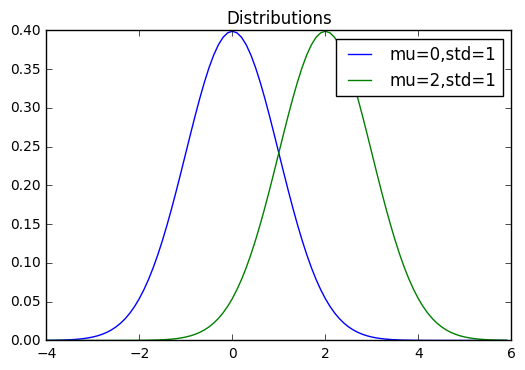
\includegraphics[scale=0.7]{histmix.png}
\end{figure}

And we can calculate the ROC curve analytically by using the probability density function of gaussian. I first had to decide the enough long interval of random variables. In case of the upper distribution I chose np.arange(-4,6,0.1). From -4 to 6 the threshold is slided with step interval 0.1. At each step the right side of the area of 1st distribution and 2nd distribution are calicurated. The right side of the area of 1st distribution divided by whole area of 1st distribution is false positive rate and The right side of the area of 2nd distribution divided by whole area of 2nd distribution is true positive rate.

\begin{verbatim}
s1 = pp1.sum()
s2 = pp2.sum()
c1 = np.cumsum(pp1)/np.cumsum(pp1)[-1]
c2 = np.cumsum(pp2)/np.cumsum(pp2)[-1]
fp = 1-c1
tp =1-c2
plt.plot(fp,tp)
plt.title("Analytical ROC")
\end{verbatim}

\begin{figure}[htbp]
  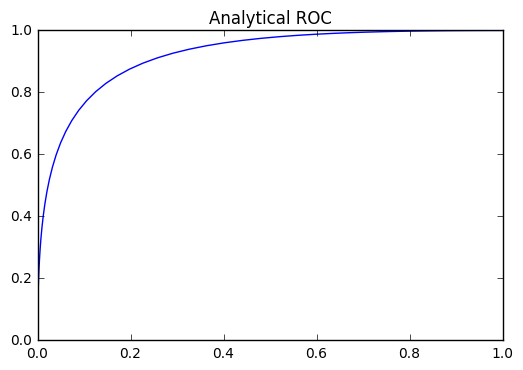
\includegraphics[scale=0.7]{roc.png}
\end{figure}

After that the empirical ROC curve is calicurated with n datasets by the following algorithum. And ploted with analytical ROC curve.

\begin{verbatim}
def ROCcul(P):
    f= np.linspace(-4,6,21)#np.arange(11)-4
    ptrue = np.array(P[:,1])
    ttp = ptrue.sum()
    tfp = len(ptrue)-ttp
    roc = np.zeros((2,len(f)))
    for i in range(len(f)):
        pred =np.zeros(len(P))
        pred[np.where(P[:,0]>f[i])]=1
        roc[1][i] = ptrue[np.where(pred==1)].sum()/ttp
        roc[0][i] = pred[np.where(ptrue==0)].sum()/tfp
    ROC=roc[:,np.argsort(roc[0])]
    return ROC

N = np.arange(1000,9000,1000)
plt.figure(figsize=(7,7))
plt.plot(fp,tp,label="Analytical ROC",linewidth=3.0)
cl = ['black','red','blue','yellow','black','red','blue','yellow']
line = ['solid','solid','solid','solid','dashed','dashed','dashed','dashed']
ite = 0
for n in N:
    p1 = np.random.randn(n/2)
    p2 = np.random.randn(n/2) +2
    P1 = np.append(p1.reshape(1,len(p1)),np.zeros((1,len(p1))),0)
    P2 = np.append(p2.reshape(1,len(p2)),np.ones((1,len(p2))),0)
    P = np.append(P1,P2,1)
    P =P.T[np.argsort(P[0])]
    ptrue = np.array(P[:,1])
    sroc = ROCcul(P)
    plt.plot(sroc[0],sroc[1], label=("Emprical n=",n),color=cl[ite],linestyle=line[ite])
    ite = ite+1
plt.legend(loc="lower right")
plt.xlabel("FP rate")
plt.ylabel("TP rate")
plt.title("ROC curve")
\end{verbatim}

\begin{verbatim}








\end{verbatim}

\begin{figure}[htbp]
  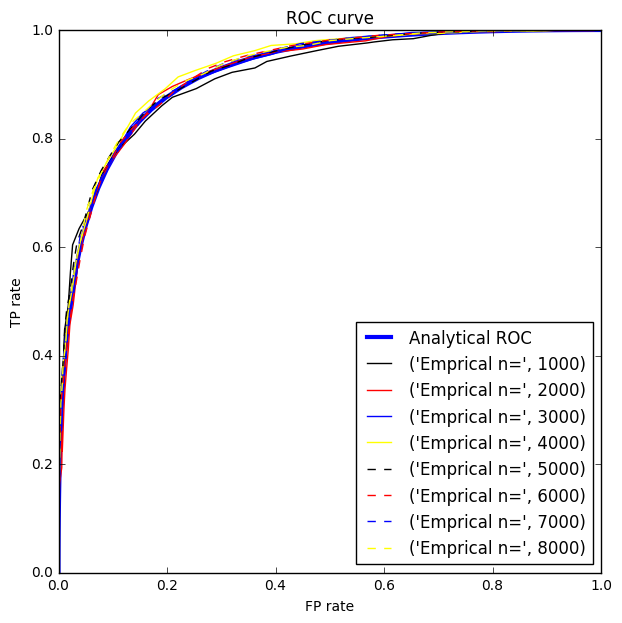
\includegraphics[scale=0.6]{rocall.png}
\end{figure}

The analytical ROC curve is much smoother than all empirical ROC curves. And it lies on middle of empirical ROC curves. In case of empirical ROC curve The more sample data points are, the clother the ROC curve seems to lie on the upper left side. But this difference is not much remarkable.

	


\section*{Assignment 4}
\subsection*{Inv or Solve}


\begin{eqnarray*}
X=
\left(
\begin{array}{cccc}
2 & 4 & 6 \\
8 & 10 & 12  
\end{array}
\right)
, \:\:\:\:
\mu = 
\left(
\begin{array}{cccc}
4  \\
10  
\end{array}
\right) 
\end{eqnarray*}
\begin{eqnarray*}
C &=&
\left(
\begin{array}{cccc}
-2 & 0 & 2 \\
-2 & 0 & 2  
\end{array}
\right) 
\left(
\begin{array}{cccc}
-2 & -2\\
0 & 0 \\
2 & 2  
\end{array}
\right) 
= 
\left(
\begin{array}{cccc}
8 & 8\\
8 & 8 \\  
\end{array}
\right) \\
&\Rightarrow& \det(C) =0
\end{eqnarray*}





\end{document}

